\documentclass[../../index]{subfiles}

\begin{document}
\chapter{\LuaLaTeX による実例}
\label{chapter:lualatex}
この章では,\LuaLaTeX による文書作成の実例を示す.
ただし,\LuaLaTeX とは\TeX エンジン\LuaTeX とマクロパッケージ\LaTeX の組み合わせを指す.

なお,文章を組版する方法については\cite{Tobias2021}に,数式を組版する方法については\cite{ams2017}と\cite{ams2018}に,それぞれ詳しく記されている.
また,検索すれば多くのWebサイトがヒットする.そこで本書では,最低限の説明に加えて,和文特有の注意点を述べるにとどめる.

また,\cite{Manuel2021}は参考になる文書を目的別に整理している.ごく簡潔であるので,この章を読む前に
目を通すことを推奨する.本書のソースはGitHubで公開されているので,それも参考にできるだろう.

\section{和文のドキュメントクラス}
\LuaLaTeX で利用でき,和文の文書作成を目的とするドキュメントクラスには,大きく次の3系統がある.

\begin{enumerate}
  \item \LuaLaTeX -ja用jsclasses互換クラス(\url{https://osdn.net/projects/luatex-ja/})
  \item BXjscls(\url{https://github.com/zr-tex8r/BXjscls})
  \item jlreq(\url{https://github.com/abenori/jlreq})
\end{enumerate}

なお,ドキュメントクラスが\LuaLaTeX に対応していれば,\inlinecode{luatexja}パッケージを読み込むことで
和文の組版に対応させられる.

本書では「1.\LuaLaTeX -ja用jsclasses互換クラス」を利用した例を示す\footnote{なお,本書そのものはjlreqを利用して作成されている.}.
\LuaLaTeX -ja用jsclasses互換クラスとは,\pLaTeX と\upLaTeX で利用できたjsclasses\index{jsclasses@jsclasses}という
ドキュメントクラス群を,\LuaLaTeX でも利用できるようにしたドキュメントクラス群である.
\inlinecode{ltjsarticle}\index{ltjsarticle@ltjsarticle},\inlinecode{ltjsreport}\index{ltjsreport@ltjsreport}などがこれに属する.

実際に使ってみる.次の内容で\inlinecode{test.tex}というファイルを作成する
\footnote{1行目の「17pt」という指定は,見本を本書に含めるときに,文字が小さくなりすぎるのを防ぐためのものであり,消して構わない.消す場合,1行目は「\texttt{\textbackslash documentclass\textbraceleft ltjsarticle\textbraceright}」となる.}.
\begin{codeblock}
\documentclass[17pt]{ltjsarticle}
% (from)
\title{表題}
\author{作者名}
\date{\today}
% (to)
\begin{document}
\maketitle
\tableofcontents
\section{節見出し}
\subsection{小節見出し}
ここに本文が入る\footnote{脚注}.

段落を変えたければ,1つ空白行を設ける.
\end{document}
\end{codeblock}

なお,\TeX では\inlinecode{%}から始まる行はコメントとして扱われ,出力に影響しない.
また,\inlinecode{% (from)}から\inlinecode{% (to)}まで,
すなわち\inlinecode{\documentclass[...]{...}}から\inlinecode{\begin{document}}の手前まで
を\termdef{プリアンブル}\index{ぷりあんぶる@プリアンブル}という.
\inlinecode{\usepackage}などはプリアンブルに記述する.

次に,コマンドラインから\LuaLaTeX を実行する.
\begin{codeblock}
> lualatex test
\end{codeblock}

すると,\cref{figure:without_toc}に示すPDFが得られる.
\cref{figure:without_toc}を見ると,目次の内容が書き込まれていないことが分かる.
その代わり,PDFがあるディレクトリに\inlinecode{test.toc}というファイルが生成されている.
このファイルには,\LaTeX ソースから構成された目次が書き込まれている.
そこで,もう一度\LuaLaTeX を実行すれば,目次が書き込まれたPDFを得られる.
\cref{figure:simple}に完全なPDFを示す.

\begin{figure}[htbp]
  \begin{subfigure}{0.5\linewidth}
    \centering
    \tcbincludegraphics[myframe,width=\smallfiguresize]{without-toc.pdf}
    \caption{\LuaLaTeX を1回実行した結果}
    \label{figure:without_toc}
  \end{subfigure}%
  \begin{subfigure}{0.5\linewidth}
    \centering
    \tcbincludegraphics[myframe,width=\smallfiguresize]{simple.pdf}
    \caption{\LuaLaTeX を2回実行した結果}
    \label{figure:simple}
  \end{subfigure}
  \caption{シンプルな和文の文書}
\end{figure}

\section{文献管理と索引作成}
通常,\LaTeX で参考文献を管理するには\BibTeX\index{bibtex@\BibTeX}というプログラムが用いられる.
また,索引を作成するにはmakeindex\index{makeindex@makeindex}というプログラムが用いられる.
しかし,これらはいずれも和文とUnicodeに対応していない.
そこで,和文の文書を作る際には,代わりにこれらの拡張版を利用するとよい.\BibTeX については\upBibTeX\index{upbibtex@\upBibTeX},
makeindexについてはupmendex\index{upmendex@upmendex}が,和文とUnicodeに対応した拡張である.

\section{\LuaLaTeX によるフォント設定}
\LuaLaTeX において,欧文フォントの変更は\inlinecode{fontspec}\index{fontspec@fontspec}パッケージにより行う.
たとえば,この文書ではプリアンブルに次のように書くことで,ソースコードのフォントを白源\footnote{\url{https://github.com/yuru7/HackGen}}に変更している.
\begin{codeblock}
\setmonofont{HackGen Regular}[BoldFont={HackGen Bold}]
\end{codeblock}

また,和文フォントの変更は\inlinecode{luatexja-fontspec}\index{luatexja-fontspec@luatexja-fontspec},
あるいは\inlinecode{luatexja-preset}\index{luatexja-preset@luatexja-preset}パッケージによって行う.

なお,フォントを変更するときは,フォントのライセンスを確認するべきである.
上記のパッケージを利用すると,初期設定ではPDFにフォントファイルの一部が埋め込まれる.
これは,設定したフォントが読者のコンピュータにインストールされていなくても,PDFを適切に表示するためである.
しかし,埋め込みの可否はフォントによって異なる.
白源は\termdef{SIL Open Font License}\index{silopenfontlicense@SIL Open Font License}という
ライセンスの下で配布されており,このライセンスは利用者に埋め込みを許可している.

\section{グラフの作成}
本書では,次の2つの方法を紹介する.
\begin{enumerate}
  \item PGFPlotsによる方法
  \item GNUPlotによる方法
\end{enumerate}

PGFPlots\index{pgfplots@PGFPlots}は,\TikZ\index{tikz@\TikZ}というパッケージを利用し,データを可視化するパッケージである.
利用方法はマニュアル\cite{christian2021}に詳しく記されているので,ここでは\cref{figure:pgfplots}に実例を示すにとどめる.

\begin{codeblock}
\begin{figure}[htbp]
  \centering
  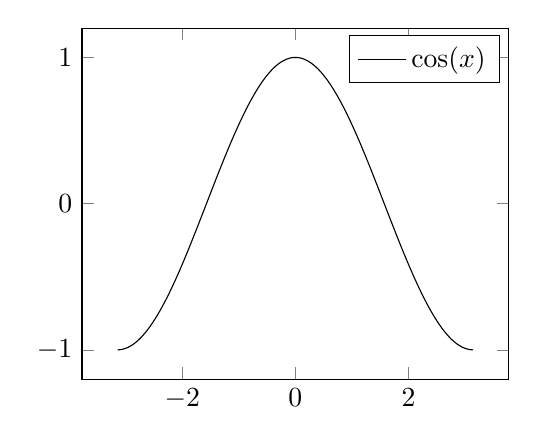
\begin{tikzpicture}
    \begin{axis}[width=7cm]
      \addplot [smooth,samples=100,domain=-pi:pi] {cos(deg(x))};
      \addlegendentry{$\cos(x)$};
    \end{axis}
  \end{tikzpicture}
  \caption{PGFPlotsによる\(\cos(x)\)のグラフ}
\end{figure}
\end{codeblock}

\begin{figure}[htbp]
  \centering
  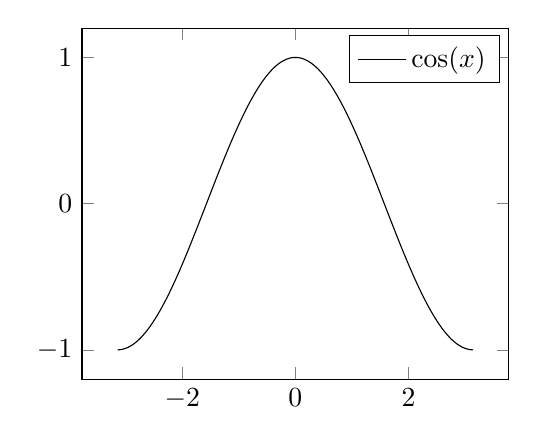
\begin{tikzpicture}
    \begin{axis}[width=7cm]
      \addplot [smooth,samples=100,domain=-pi:pi] {cos(deg(x))};
      \addlegendentry{$\cos(x)$};
    \end{axis}
  \end{tikzpicture}
  \caption{PGFPlotsによる\(\cos(x)\)のグラフ}
  \label{figure:pgfplots}
\end{figure}

GNUPlot\index{gnuplot@GNUPlot}は,関数やデータを描画するプログラムである.
公式サイト(\url{http://www.gnuplot.info/})からダウンロードできる.
こちらも,利用方法は公式サイトに詳しく記されているので,\cref{figure:gnuplot}に実例を示すにとどめる.

まず,\LaTeX ソースがあるディレクトリに移動する.
その後,コマンドラインでGNUPlotを起動し,以下のように入力する
\footnote{1行目を\texttt{set term tikz}としている資料もあるが,これは\texttt{set terminal lua tikz}の省略形である.}.

\begin{codeblock}
gnuplot> set terminal lua tikz size 7cm,5cm
gnuplot> set output "gnuplot.tex"
gnuplot> set xrange [-pi:pi]
gnuplot> plot cos(x) linetype rgb "black" title '$\cos(x)$'
gnuplot> exit
\end{codeblock}

すると,カレントディレクトリにいくつかのファイルが出力される.
プリアンブルに\inlinecode{\usepackage{gnuplot-lua-tikz}}を追加し,
\LaTeX ソースに次の記述を加える.すると,\cref{figure:gnuplot}のグラフが得られる.

\begin{codeblock}
\begin{figure}[htbp]
  \centering
  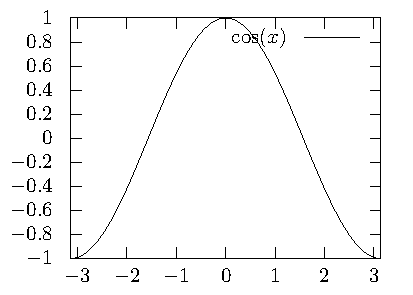
\includegraphics{gnuplot.pdf}
  \caption{GNUPlotによる\(\cos(x)\)のグラフ}
\end{figure}
\end{codeblock}

\begin{figure}[htbp]
  \centering
  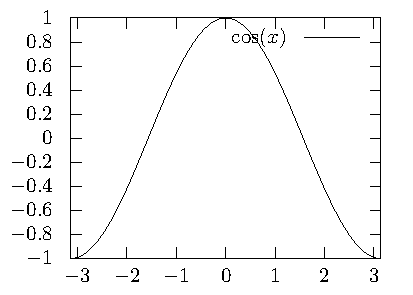
\includegraphics{gnuplot.pdf}
  \caption{GNUPlotによる\(\cos(x)\)のグラフ}
  \label{figure:gnuplot}
\end{figure}

3Dグラフなども同様の要領で作成できる.以下にPGFPlotsを利用した例を示す.

\begin{codeblock}
\begin{figure}[htbp]
  \centering
  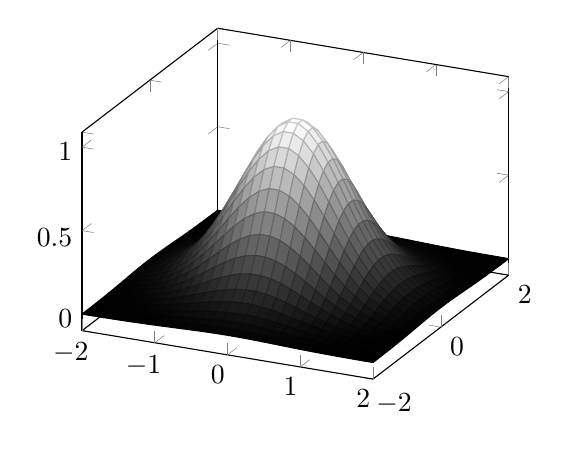
\begin{tikzpicture}
    \begin{axis}[width=7cm,colormap/blackwhite]
      \addplot3 [surf,miter limit=1,samples=30,domain=-2:2] {exp(-(x^2+y^2))};
    \end{axis}
  \end{tikzpicture}
  \caption{\(e^{-(x^2+y^2)}\)のグラフ}
\end{figure}
\end{codeblock}

\begin{figure}[htbp]
  \centering
  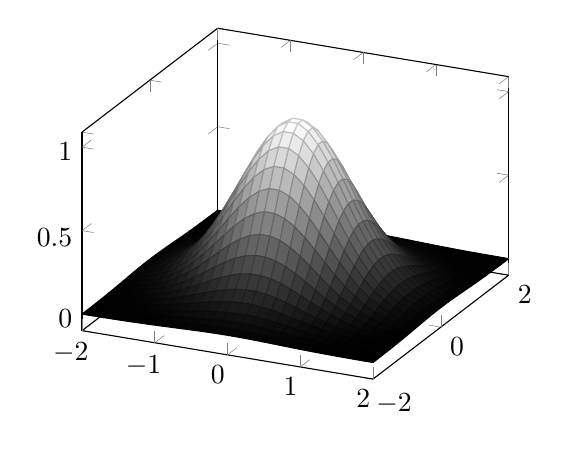
\begin{tikzpicture}
    \begin{axis}[width=7cm,colormap/blackwhite]
      \addplot3 [surf,miter limit=1,samples=30,domain=-2:2] {exp(-(x^2+y^2))};
    \end{axis}
  \end{tikzpicture}
  \caption{\(e^{-(x^2+y^2)}\)のグラフ}
\end{figure}

\section{補遺}
\subsection{他の命令の引数にできない命令}
\TeX の仕様により,\inlinecode{\verb}など一部の命令は,他の命令の引数にできない.
たとえば,次の\LaTeX ソースは\inlinecode{\verb}が
\inlinecode{\footnote}の引数になっているので不正である.
\begin{codeblock}
\documentclass[uplatex,dvipdfmx]{jsarticle}
\begin{document}
\TeX のロゴ(\emph{\verb!\TeX!で出力できる})は,Donald Knuthがこう表記するように求めている.
\end{document}
\end{codeblock}

実際,\inlinecode{example.tex}を上記の内容で作成し,
次のコマンドを実行すると「\inlinecode{LaTeX Error: \verb illegal in command argument.}」というエラーが出力される.
\begin{codeblock}
> uplatex -kanji=utf8 -no-guess-input-enc example
\end{codeblock}

この問題を解決する手っ取り早い方法は,\inlinecode{\verb}を使わないことである.
すなわち,\textbackslash を\inlinecode{\textbackslash}に置き換えればよい.
\begin{codeblock}
\documentclass[uplatex,dvipdfmx]{jsarticle}
\begin{document}
\TeX のロゴ(\emph{\texttt{\textbackslash TeX}で出力できる})は,Donald Knuthがこう表記するように求めている.
\end{document}
\end{codeblock}

\end{document}
